\section{Introduction}
An electrocardiogram (EKG or ECG) is a test used to check the problems with the electrical activity of heart. Human heart works with an periodic electrical pulse which is used to contract and expand the heart mussels according to generated polarity. These electrical signals can be captured placing electrodes in specific locations of the human body. Then the captured electrical signals can be analyses to detect the irregularities of heart called arrhythmia.  A normal ECG signal is a periodic signal of having around 72 cycles per minute. Figure \ref{ecg_signal} shows a typical ECG waveform signal.
\begin{figure}
        \centering
        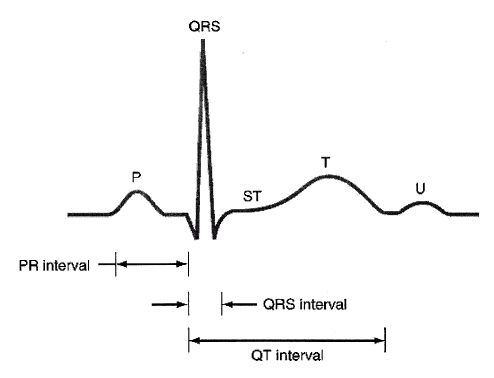
\includegraphics[width=\textwidth]{ecg_signal.png}
        \caption{Normal ECG Signal}
        \label{ecg_signal}
\end{figure}
